
\documentclass[a4paper,10pt,article,oneside,english]{memoir} 
% DANSK OPSÆTNING
\usepackage[english]{babel}
\usepackage[utf8]{inputenc}
\usepackage[T1]{fontenc}
\usepackage{lmodern} 
\renewcommand{\englishhyphenmins}{22} 


% FIGURER
\usepackage{graphicx}

% MATEMATIK
\usepackage{amsmath}
\usepackage{amssymb,amsthm,bm}
\usepackage{mathtools}	


% This document uses
\usepackage[draft,silent]{fixme}
\usepackage{hyperref}
\usepackage{siunitx}


% captions in italic
\let\oldcaption\caption
\renewcommand{\caption}[1]{\oldcaption{\emph{#1}}}


\begin{document}
	%\frontmatter
	%\clearpage	
	%\tableofcontents*
	\title{Machine Learning E16 - Handin 2\\OCR with SVM and (Deep) Neural Networks}
	\author{Mark Medum Bundgaard, Morten Jensen, Martin Sand Nielsen}
	\date{\today, Aarhus University}
	
	\mainmatter
	\maketitle
	
	
	
	\chapter{SVM with SciKit-Learn}
	Several Support Vector Machine-classifier has been trained on the \emph{AUtrain}-digits with different kernels. See Table \ref{tab:svm_accuracy} for the achieved classification results. The implementation of SVMs from Scikit-learn  \footnote{ \url{http://scikit-learn.org/stable/modules/generated/sklearn.svm.SVC.html}}
	is used for these experiments.
	
	\section{Polynomial kernels}
	A linear(1st order polynomial), a 2nd and 3rd order polynomial has been trained with various values for the hyperparameter, $C$. This parameter defines how much it should cost for each support vector, that is not kept outside the SVM margins. Too large $C$ and the SVM will tend to overfit the training data to avoid any support vectors in margins. Too low $C$ results in no penalty for not fitting the training data well. The optimal value for this hyperparameter is found by evaluation with a separate validation set. See the comparison of these \emph{in sample} and \emph{out of sample} classification accuracies for various $C$ values in Figure \ref{fig:svm_lin}, \ref{fig:svm_poly2} and \ref{fig:svm_poly3}.
	
	\begin{figure}[h!]
		\centering
		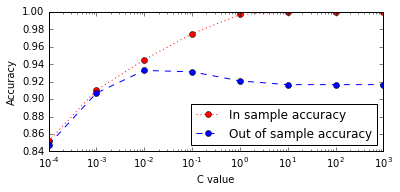
\includegraphics[width=0.7\linewidth]{svm_lin.PNG}
		\caption{SVM performance with a simple linear(1st order polynomial) kernel for various $C$  values(cost).}
		\label{fig:svm_lin}
	\end{figure}
	
	\begin{figure}[h!]
		\centering
		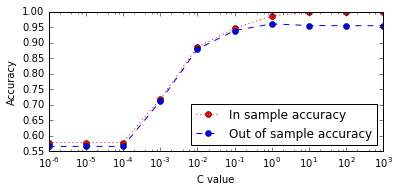
\includegraphics[width=0.7\linewidth]{svm_poly2.PNG}
		\caption{SVM performance with a second-order polynomial kernel for various $C$ values(cost).}
		\label{fig:svm_poly2}
	\end{figure}
	
	\begin{figure}[h!]
		\centering
		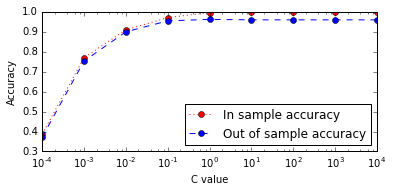
\includegraphics[width=0.7\linewidth]{svm_poly3.PNG}
		\caption{SVM performance with a third-order polynomial kernel for various $C$ values(cost).}
		\label{fig:svm_poly3}
	\end{figure}
	
	
	
	
	
	
	
	
	\section{RBF kernel}
	A more general kernel that is often used, is the Radial Basis Function (RBF).
	Which expands the raw input feature dimensions (vector of pixel values) to infinite many feature dimensions, such that they results in a similarity measure between images. Beside the usual $C$ cost hyper parameter, RBF also has a $\gamma$ hyper parameter defining the width of the bell shape for each data point(image).
	
	
	The results of a coarse grid search for the optimum combination of these parameters can be seen in Figure \ref{fig:svm_rbf_grid}. 
	For comparing the RBF kernel with the polynomial kernels, the optimal $\gamma=0.01$ has been used in Figure \ref{fig:svm_rbf}.
	
	\begin{figure}[h!]
		\centering
		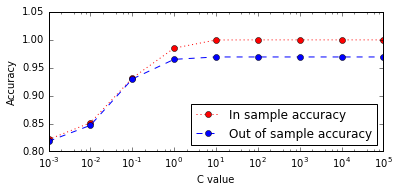
\includegraphics[width=0.7\linewidth]{svm_rbf.PNG}
		\caption{SVM classification accuracy with a RBF kernel with $\gamma=0.01$ for various $C$ values(cost).}
		\label{fig:svm_rbf}
	\end{figure}
	
	\begin{figure}[h!]
		\centering
		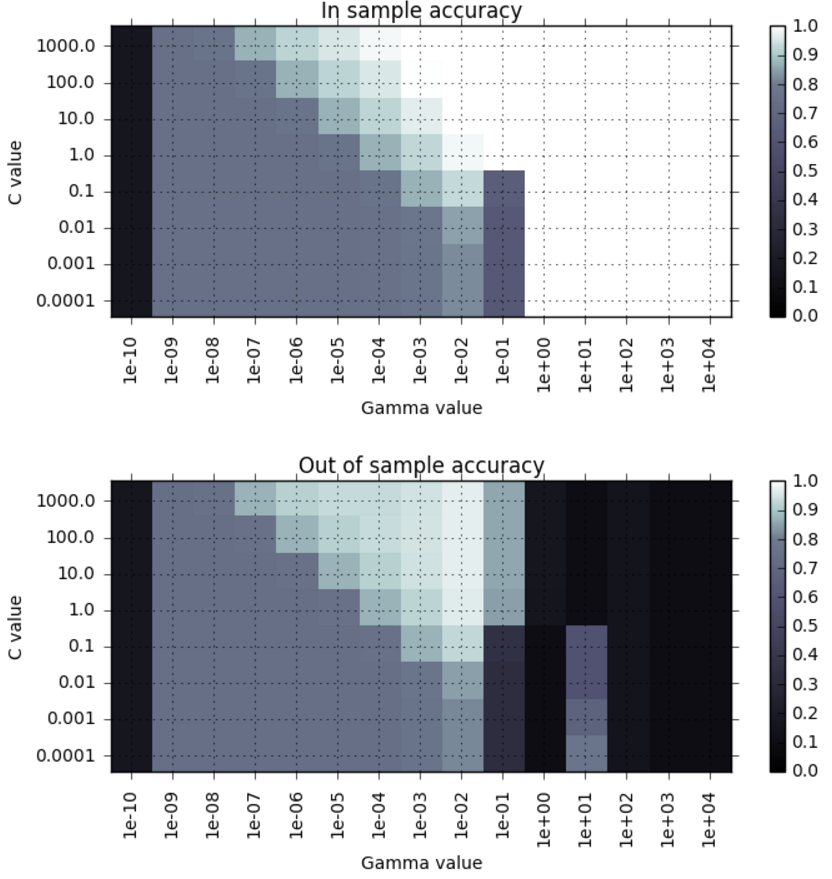
\includegraphics[width=0.9\linewidth]{svm_rbf_grid.PNG}
		\caption{SVM classification accuracy with a RBF kernel with various $\gamma$- and $C$ values(cost).}
		\label{fig:svm_rbf_grid}
	\end{figure}
	
	A comparison of the kernels can be found in Table \ref{tab:svm_accuracy}. RBF is the best with a validation classification accuracy of $96.94\%$. The search for hyper parameters was only coarse with big step sizes, so there is clearly room for improvements. A better parameter search has to be evaluated by yet another separate validation set, so as to avoid overfitting the hyper parameters to the validation set. 
	
	The two dimensional hyper parameter fit for RBF results in many more SVM trainings. In some situations a less complex kernel with faster training time would be preferable.
	
	\begin{table}[h!]
		\centering
		\caption{Classification accuracy with different kernels for the found optimal hyperparameters. }
		\label{tab:svm_accuracy}
		\begin{tabular}{crr S[table-format=2.4]}
			SVM kernel & Validation accuracy & Training accuracy & {$C$-value} \\ 
			\hline 
			Linear & $93.29\%$ & $94.52\%$ & 0.01 \\ 
			2nd order poly. & $96.16\%$ & $98.74\%$ & 1 \\ 
			3rd order poly. & $96.28\%$ & $99.73\%$ & 1 \\ 
			RBF ($\gamma=0.01$) & $96.94\%$ & $99.98\%$ & 10 \\ 
		\end{tabular} 
	\end{table}
	
	
	
	
	
	
	
	
	
	
	\chapter{Neural Nets with TensorFlow}
	The TensorFlow\footnote{\url{https://www.tensorflow.org/}} computation library has been used for implementing two neural networks. 
	
	A simple neural network (NN) with one hidden fully connected layer (and an input and output layer) has been implemented. See Figure \ref{fig:nn_layout}. The input images is represented by a feature vector of size 784 equal to the number of pixels. The hidden layer has 1024 fully connected nodes, with weight-matrix and biases-vector as parameters. The fully connected output layer consists of 10 nodes with a dropout rate of $0.5$. The dropout can introduce a redundancy so that no single node in the hidden layer is indicator for one output class. No dropout is performed when evaluating the network.
	
	\begin{figure}[h!]
		\centering
		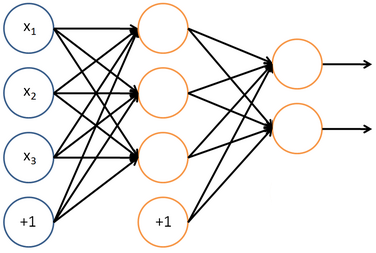
\includegraphics[width=0.4\linewidth]{nn_layout.png}
		\caption{Illustration of a small NN, with one hidden layer. In our case the input vector consists of the $784$ pixel values for an image, the hidden layer has $1024$ nodes, and the output layer has $10$ nodes, one for each digit-class. Biases are added for both computational layers.}
		\label{fig:nn_layout}
	\end{figure}
	
	
	
	\section{Improved (combined) training set}
	To improve training, the AUtrain and MNIST dataset have been combined into one for training. The training set of $65000$ images should be even more resistant to over fitting the CNN during training. 
	The original AUtest set is still used for validation while finding the optimal hyper parameters. Then for the final model training, when the best model is chosen, the test set is included in the training set before deploying the model for prediction of digits.  
	
	
	\section{Training}
	The training was done with TensorFlow on GPU with a batchsize of 512. For every 100 iterations an evaluation of the accuracy was performed. 
	The learning rate was set as a exponetial decresing learning rate, starting at $0.001$ and dropping by a factor of $0.96$ every $100$ iterations. The parameters was randomly initialized by standard procedures.
	
	Furthermore a snapshot of the layer parameters was saved when evaluating the model. When no increase in out of sample accuracy is observed the training is stopped. Maximum number of iterations was set at $10000$ to leave the computations overnight. The snapshot corresponding to the highest accuracy is saved, and now define the final trained model. The validation accuracy of the trained neural network was $96.47\%$ at iteration 3200. No sign of significant overfitting occured. See Figure \ref{fig:nn_learning}. 
	
	\begin{figure}[h!]
		\centering
		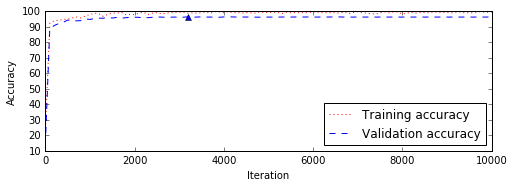
\includegraphics[width=0.9\linewidth]{nn_learning.png}
		\caption{Learning curve for the simple neural network. The triangle marks maximum.}
		\label{fig:nn_learning}
	\end{figure}
	
	
	
	
	
	
	
	
	\chapter{Making the best classifier in 2016 ML Class}
	In an attempt to make a even better classifier the simple neural network has been expanded by adding two convolution layers and max pooling layers before the two fully connected layers. See Figure \ref{fig:cnn_layout}.
	
	\begin{figure}[h!]
		\centering
		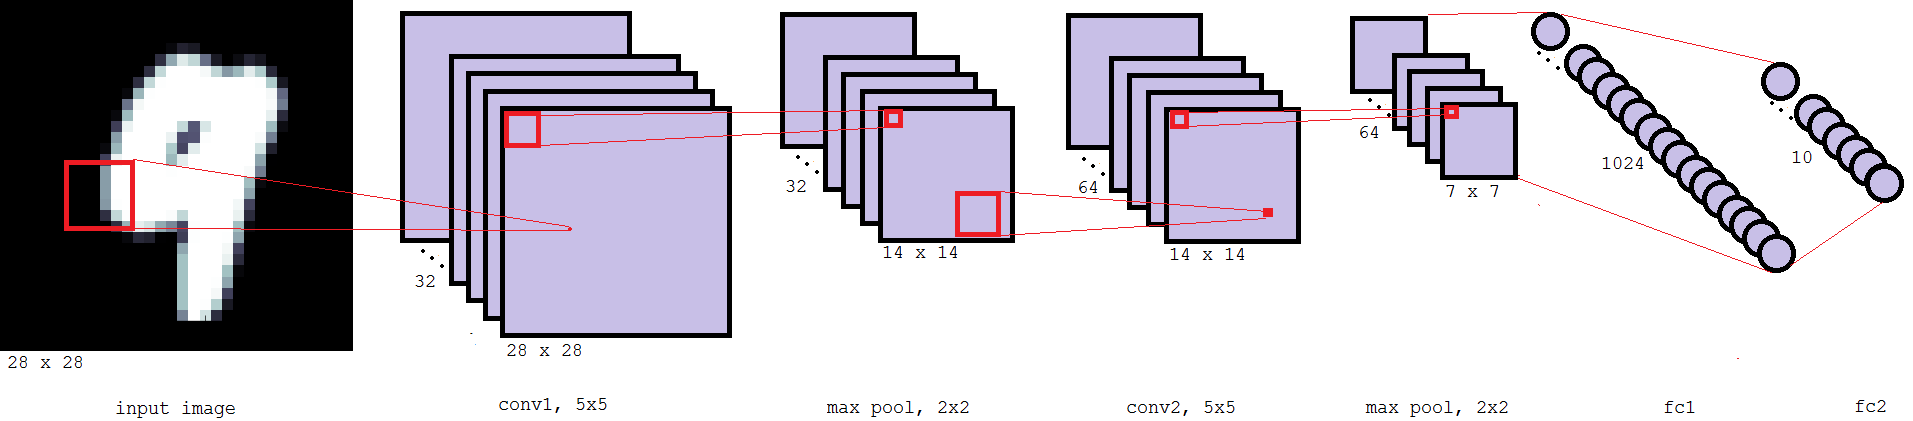
\includegraphics[width=0.9\linewidth]{cnn_layout.png}
		\caption{Illustration of the CNN. Two $5 x 5$ convolution layers and $2 x 2$ max pooling layers before a fully connected layer of $1024 nodes$ and the fully connected output layer of $10$ nodes. Input monochrome images of $28x28$ pixels assumed.}
		\label{fig:cnn_layout}
	\end{figure}
	
	The input feature(pixel) vector is reshaped to a two dimensional matrix. The first convolution has $32$ filters with size $5x5$ with stride $1$. Padding is used to allow convolutions on the outer parts of the image and keep resolution. A max pool layer over $2x2$ areas effectively halves the resolution before yet another similar convolution with $64$ filters. A similar max pool reduce the data to $7x7x64$ scalars. Then a fully connected layer of $1024$ nodes and a output layer with dropout rate $0.5$ similar to the previously explained simple NN takes the convolution layer output into outputs for the 10 classes. 
	
	
	
	
	\section{Training}
	Training was performed like the the simple neural network, but with a factor $0.94$ in learning rate every $100$ steps. The learning progression is plotted in Figure \ref{fig:cnn_learning}. 
	The maximum validation accuracy of $98.22\%$was reached at $2300$ iterations.
	This result can be compared to the other models in Figure \ref{tab:classifier_accuracy}. 
	
	\begin{figure}[h!]
		\centering
		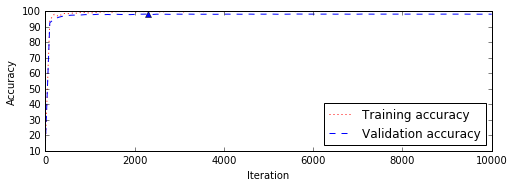
\includegraphics[width=0.9\linewidth]{cnn_learning.png}
		\caption{Learning curve for the convolution neural network. The triangle marks maximum.}
		\label{fig:cnn_learning}
	\end{figure}
	
	
	
	
	
	\begin{table}[h!]
		\centering
		\caption{Classification accuracy for the RBF kernel SVM, simple neural network with one hidden layer, and convolution neural network, all trained on the combined AUtrain and MNIST set, and validated with AUtest. }
		\label{tab:classifier_accuracy}
		\begin{tabular}{lr}
			Classifier & Validation accuracy \\ 
			\hline 
			SVM with RBF & $96.78\%$ \\ 
			NN & $96.47\%$ \\ 
			CNN & $98.22\%$ 
		\end{tabular} 
	\end{table}
	
	
	
	
	
	
	\chapter{Discussion}
	The final model deployed as a classifier in the delivered predict.py is the CNN trained on all data sets readily available as one combined training set. Therefore this final model has not been validated with any dedicated test set, but we trust that th dropout during training and stopping at iteration 4000(early stopping) will avoid overfitting. The actual effect of dropout has not been subject to experiment for this report. 
	
	A lot of hyper parameters has not been explored in our work. Size and quantity of layers, and different combination of layers could have huge influence on training speed and generalization of the final classifier network. More advanced schemes for validation could probably also have improved our training. 
	But the experiments truly shows that neural networks outperforms the most used SVM and kernel combinations.
	
	
	
	
\end{document}
